\section{The Application-Level Crash\\ Explorer (ALICE)}
\label{sec-tool}

We have now seen that file systems provide different persistence properties.
However, some important questions remain: How do current applications update
their on-disk structures? What assumptions do they make about the underlying
file systems? Are such update protocols correct?

To gain insight into these questions, we develop the {\em Application-Level
  Crash Explorer (\toolname)}, a framework that analyzes application update
protocols and discovers crash vulnerabilities. \toolname\ detects
vulnerabilities by testing whether the application is vulnerable to violations
of various persistence properties.

We first describe the mechanism used by \toolname\ to test a persistence
property. We then describe the policy used by \toolname: what persistence
properties to test. We discuss how vulnerabilities are reported, a few details
of the tool implementation, and finally its limitations.

\begin{figure}[!t]
\centering
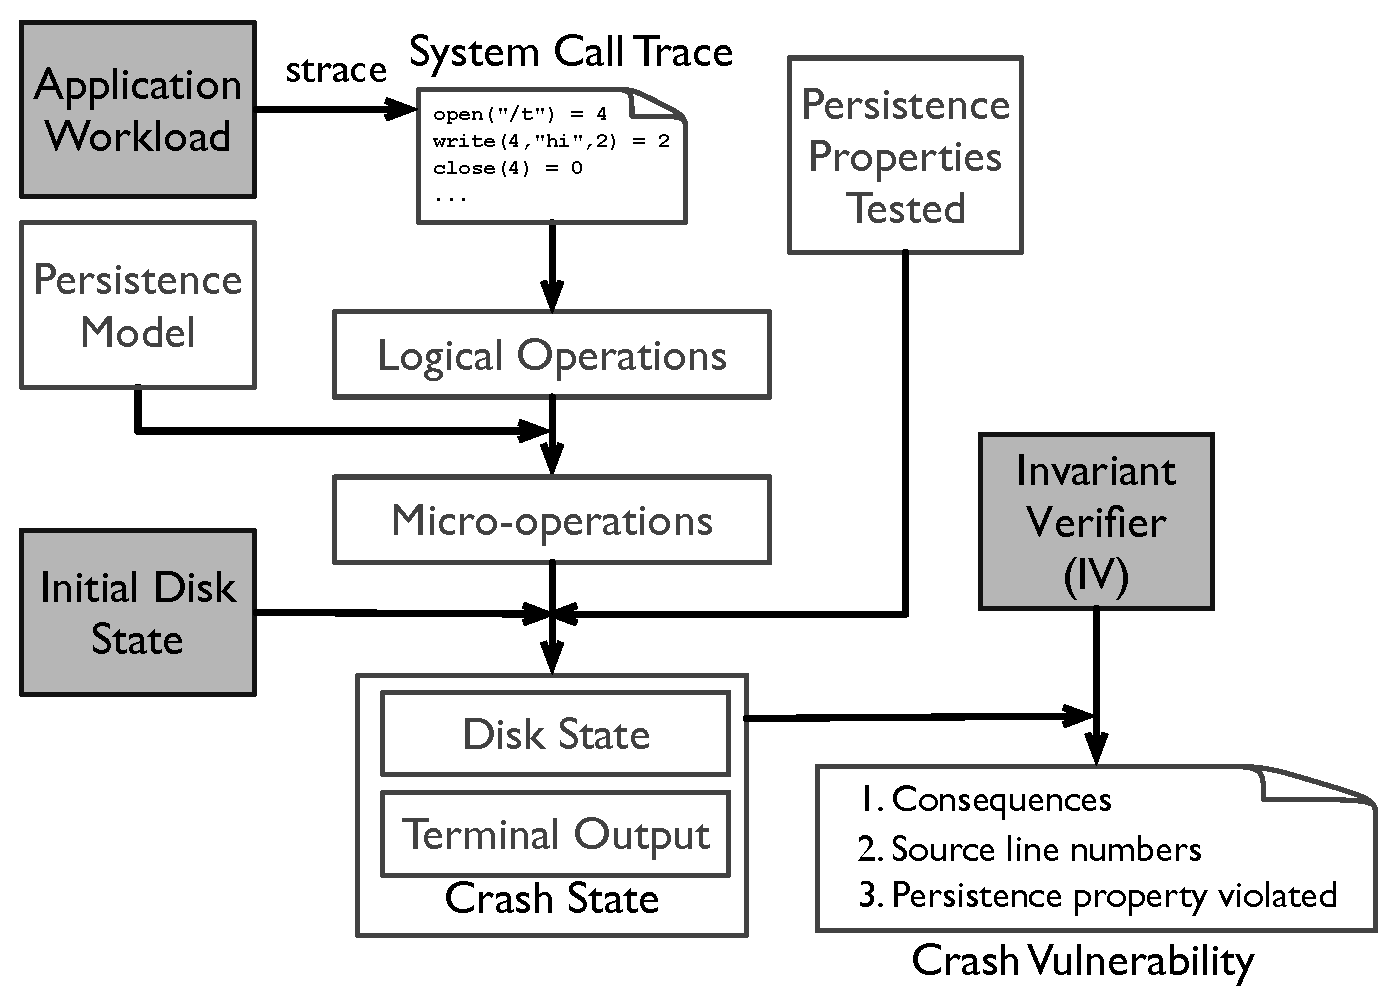
\includegraphics[scale=0.28]{figs/overview2.eps}
\mycaption{fig-overview}{Detecting Vulnerabilities using \toolname}{\footnotesize The
figure shows an overview of how \toolname\ converts user inputs into crash states and
finally into crash vulnerabilities. The shaded grey boxes are inputs supplied by the user.}
\end{figure}




\subsection{Testing a Persistence Property}

To test whether the application depends on a particular persistence property
(e.g., write atomicity), \toolname\ \textit{violates} that persistence
property (e.g., breaks a write into many parts), and generates the
corresponding possible on-disk crash states.  \toolname\ then checks whether
application invariants are violated for each crash state.

Violating a single persistence property can lead to many crash states. For
example, if append atomicity is violated, a file can end up with either a
prefix of the data persisted, with random data intermixed with file data, or
various combinations thereof. We use a \textit{file-system persistence model}
to define the exact intermediate states possible when persistence properties
are violated.

Figure~\ref{fig-overview} shows an overview of how \toolname\ finds crash
vulnerabilities. For each application to be tested, the user supplies a
workload exercising that application, and an invariant verifier to check
application invariants.  \toolname\ runs the application and collects the
resulting system-call trace.  \toolname\ first converts system calls into
logical operations, then converts these logical operations into {\em
micro-operations} as per the persistence model. \toolname\ then uses
micro-operations to generate crash states.  \toolname\ finally runs the
application on each crash state and uses the invariant verifier to check if the
application is inconsistent. We now discuss these steps in more detail.

\subsubsection{Logical Operations}

\toolname\ first converts the trace of system calls in the application
workload to \textit{logical operations}. Logical operations abstract away
details such as file descriptors and current read and write offsets, and
transform a large set of system calls and other I/O producing behavior into a
small set of file system operations. For example, \smalltt{write()},
\smalltt{pwrite()}, \smalltt{writev()}, \smalltt{pwritev()} and writes to
\smalltt{mmap()}-ed regions are all translated into \smalltt{overwrite} or
\smalltt{append} logical operations. Logical operations are used to
produce the protocol diagrams shown in Section~\ref{sec-intro} and
Section~\ref{sec-case}.

\subsubsection{File-System Persistence Model}

\begin{table}[!t]
%\vspace{0.1in}
\begin{center}
{\footnotesize
\begin{tabular}{c|l}
\textbf{Logical Operation} & \textbf{Micro-operations} \\
\hline
overwrite &     $N \times$ write\_block(data) \\
\hline
append  &       $N \times$ change\_file\_size \\
        &       $N \times$ write\_block(random) \\
        &       $N \times$ write\_block(data) \\
\hline
truncate &      $N \times$ change\_file\_size \\
        &       $N \times$ write\_block(random) \\
        &       $N \times$ write\_block(zeroes) \\
\hline
link    &       create\_dir\_entry \\
\hline
unlink  &       delete\_dir\_entry \\
\hline
delete  &       change\_file\_size \\
\hline
rename &        create\_dir\_entry \\
       &        delete\_dir\_entry \\
\hline
write to terminal & stdout \\
\end{tabular}
}
\end{center}
\vspace{-0.1in}
\mycaption{tbl-log-microcode}{Translating logical operations into
micro-operations}{\footnotesize The table 
shows how logical operations such as append are translated into
micro-operations. $N$
indicates the logical operation may be broken up into many block-sized
micro-operations.
} 
\end{table}
 

\begin{lstlisting}[float=t, caption = {\textbf{Annotated Update Protocol.}
\textit{\footnotesize The
listing shows an example update protocol. The micro-operations generated for each
system call are shown along with their dependencies. The inode number of \smalltt{x2VC} 
is 12. The inode number of the root directory is 2. Some details of listed system
calls have been elided for brevity.
}}, label = {lst-micro-example}, escapechar=!]

!\vspace{-0.4in}!

open(path="/x2VC") = 10
!{\fontfamily{Times}\selectfont Micro-operations: None!
!{\fontfamily{Times}\selectfont Dependencies: None!

!\vspace{-0.2in}!
pwrite(fd=10, offset=0, size=1024)
!{\fontfamily{Times}\selectfont Micro-operations:!
!{\fontfamily{Times}\selectfont \#1 write\_block(inode=12, offset=0, size=512)}! 
!{\fontfamily{Times}\selectfont \#2 write\_block(inode=12, offset=512, size=512)}! 
!{\fontfamily{Times}\selectfont Dependencies: None!

!\vspace{-0.2in}!
fsync(10)
!{\fontfamily{Times}\selectfont Micro-operations: None!
!{\fontfamily{Times}\selectfont Dependencies: None!

!\vspace{-0.2in}!
pwrite(fd=10, offset=1024, size=1024)
!{\fontfamily{Times}\selectfont Micro-operations:!
!{\fontfamily{Times}\selectfont \#3 write\_block(inode=12, offset=1024, size=512)}! 
!{\fontfamily{Times}\selectfont \#4 write\_block(inode=12, offset=1536, size=512)}! 
!{\fontfamily{Times}\selectfont Dependencies: \#1, \#2!

!\vspace{-0.2in}!
link(oldpath="/x2VC", newpath="/file")
!{\fontfamily{Times}\selectfont Micro-operations:!
!{\fontfamily{Times}\selectfont \#5 create\_dir\_entry(dirinode=2, entry=``file", inode=12)! 
!{\fontfamily{Times}\selectfont Dependencies: \#1, \#2!

!\vspace{-0.2in}!
write(fd=1, data="Writes recorded", size=15)
!{\fontfamily{Times}\selectfont Micro-operations:!
!{\fontfamily{Times}\selectfont \#6 stdout("Writes recorded")! 
!{\fontfamily{Times}\selectfont Dependencies: \#1, \#2!

\end{lstlisting}



The {\em persistence model} defines the atomicity and ordering persistence
properties of logical operations, thus defining which crash stats are
possible. The persistence model should be sufficiently flexible to model any
modern file system. Therefore, the model is constructed based on a minimally
POSIX compliant, ext2-like file system, but can be readily changed to mimic
modern file systems such as ext4 or btrfs. 

%The model is deterministic: the
%crash state changes in response to logical operations. We make the simplifying
%assumption that the effect of any operation is restricted to its arguments: if
%we unlink $X$, $Y$ should not disappear.\footnote{Surprisingly, this is not
%  always true; in ext2, for example, unlinking one file can lead to the
%  disappearance of another unrelated file.} Without this restriction, it is
%hard to model changes to disk state in response to external operations. With
%the exception of ext2, all other file systems we study adhere to this
%behavior.

The model has three classes of logical entities: {\em file inodes}, {\em
directory entries}, and {\em data blocks}. Each logical operation operates on
one or more of these entities. An infinite number of instances of each logical
entity exist, and they are not allocated or de-allocated by logical operations,
but rather simply changed.

To capture intermediate states, the model breaks logical operations further
down into \textit{micro-operations}, i.e., the smallest atomic modification
that can be performed upon each logical entity. There are four such micro-ops: 
\begin{itemize}[topsep=0pt, itemsep=-1ex, partopsep=1ex, parsep=1ex]
\item \textit{write\_block}: an atomic write of size \textit{block} to a
  file. Two special arguments to \textit{write\_block} are \textit{zeroes} and
  \textit{random}: \textit{zeroes} indicates the file system initializing a
  newly allocated block to zero; \textit{random} indicates an uninitialized
  block with old file contents
\item \textit{change\_file\_size}: atomically increases or decreases the size
  of a file
\item \textit{create\_dir\_entry}: atomically creates a directory entry
\item \textit{delete\_dir\_entry}: atomically delete a directory entry
\end{itemize}

The atomicity properties defined by the model control what micro-operations
constitute a logical operation. Ordering properties control which
micro-operations can reach disk before other micro-operations. We first
describe how the model handles each property, and then illustrate with the
update protocol shown in Listing~\ref{lst-micro-example}.

\textbf{Atomicity}. Table~\ref{tbl-log-microcode} shows how logical file
system operations are broken into micro-ops. Overwrites and appends can be
atomic at different granularities: the smallest atomic write is of size one
byte. For example, in Listing~\ref{lst-micro-example}, the model's block size
is 512 bytes: hence, each \smalltt{pwrite()} is broken into 512 byte-sized
\textit{write\_block} operations. The append and truncate operations increase
(or decrease) the file size, and fill the extended file region with new data
(zeroes in the case of truncate). The \textit{random} and \textit{zeroes}
options of \textit{write\_block} represent uninitialized and
zeroed blocks. If the last link to a file is removed via unlink, the file is
deleted. Renaming a file is broken down into a non-atomic pair of unlink and
link operations.

\textbf{Ordering}. In the model, all operations following a sync operation on
file $A$ depend upon writes to file $A$ preceding the sync operation. For
example, in Listing~\ref{lst-micro-example}, the \#3 and \#4
\textit{write\_block} operations depend upon the \#1--2 \textit{write\_block}
operations due to the intervening \smalltt{fsync()}. Therefore, \toolname\ will
not construct a crash state that has operations \#3 or \#4 without operations
\#1 or \#2. 

\textbf{Durability}. The application may guarantee certain state to be durable
after some terminal output. To check for this in a crash state, we add a special
micro-op termed \textit{stdout}, that captures writes by the application to
terminal output. These micro-ops depend upon writes synced by preceding sync
operations. All operations following the stdout operation depend on it. In
Listing~\ref{lst-micro-example}, terminal output is represented as a
\textit{stdout} micro-op. Since it depends only on micro-ops \#1--2, a crash
state could contain the effects of \#1--2 and the \textit{stdout}
operation. If the application guarantees that the terminal message indicates all writes
(including \#3--4) are durable, this is a durability violation.

\subsubsection{Constructing and Checking a Crash State}
\label{sec-construct}

Micro-operations are generated according to the persistence model. Based on
persistence property being tested, \toolname\ selects micro-operations to be
applied in sequence to the initial crash state to generate a new crash state.

A user-supplied \textit{Invariant Verifier (IV)} is run on each crash state to
check if the application is consistent (e.g., that puts are ordered for the \smalltt{LevelDB}
asynchronous-put workload). The IV
also uses terminal output to verify durability for certain applications. If
the IV finds an invariant is violated, a vulnerability has been found. %The IV
%does further operations to find out the consequence of the vulnerability
%(e.g., all further writes to the application fail).

\subsection{Persistence Properties Tested}
\label{sec-pptested}
We now describe the different persistence properties tested by \toolname, and how
each property is tested.

\textbf{Atomicity \textit{across} System Calls}. The application update
protocol may require multiple system calls to be persisted together atomically.
This property is easy to check: if the protocol has $N$ system
calls, \toolname\ constructs one crash state for each prefix (first $X$ system
calls $\forall\ 1 < X < N$) applied. In the sequence of crash states generated
in this manner, the first crash state to have an application invariant violated
indicates the start of an atomic group. The invariant will hold once again in
crash states where all the system calls in the atomic group are applied. If
\toolname\ determines that a system call $X$ is part of an atomic
group, it does not test whether the protocol is vulnerable to $X$ being
persisted out of order, or being partially persisted.    

\textbf{System-Call Atomicity}. The protocol may require a single system call
to be persisted atomically. \toolname\ tests this for each system call by
applying all previous system calls to the crash state, and then generating 
crash states corresponding to different intermediate states of the system
call, and checking if this results in application invariants being violated.
The intermediate states for file-system operations are listed in
Table~\ref{tbl-log-microcode}. Appends have an intermediate state where the
block is filled with random data. In terms of splitting a system call into
smaller micro-operations, the write, append, and truncate operations are
handled in two ways: split into \textit{block} sized micro-operations, and
split into three micro-ops irrespective of the size of the resulting micro-op.

\textbf{Ordering Dependency among System Calls}. The protocol requires system
call $A$ to be persisted before $B$ if a crash state with $B$ applied (and not
$A$) violates application invariants. \toolname\ tests this for each pair of
system calls in the update protocol by applying every system call from the
beginning of the protocol till $B$ except for $A$. 

\subsection{Static Vulnerabilities}
Consider an application issuing ten writes in a loop. The update protocol would
then contain ten \smalltt{write()} system calls. If each write is required to
be atomic for application correctness, \toolname\ detects that \textit{each}
system call is involved in a vulnerability; we term these as \textbf{dynamic}
vulnerabilities. However, the cause of all these vulnerabilities is a single
source code line. \toolname\ uses stack trace information to correlate all
10 system calls to the source line, and reports it as a single
\textbf{static} vulnerability. In the rest of this paper, we only discuss static
vulnerabilities.

Our estimate of static vulnerabilities is conservative.  In most applications,
the source line in the inner-most stack frame points to a wrapper to the
C-library; hence we manually examine the stack to find a representative
application source line. However, when not sure about the representative frame,
we choose inner frames rather than outer ones.

\if 0
If each write is required
to be atomic for application correctness, \toolname\ would detect this 

The same
source code line can be involved in several dynamic vulnerabilities: for
example, a loop issuing 10 writes, each of which need to be atomic, would
result in 10 dynamic vulnerabilities, and a single static vulnerability. 

When \toolname\ determines that the application is vulnerable to a particular
persistence property being violated, it reports details of the vulnerability:
the exact system calls involved, the type of the vulnerability (e.g., atomicity
across system calls, ordering, etc.), and the consequences of the vulnerability
(e.g., corruption). We term this a \textbf{dynamic} vulnerability.
\toolname\
takes care not to over-report dynamic vulnerabilities: every system call in the
update protocol that must be atomically persisted is reported once; every group
of system calls that must be atomically persisted is reported once; every pair
of system calls $A$ and $B$ where $A$ must be persisted before $B$ is reported
once.  

Using \toolname\ and the system call stack trace, we can correlate dynamic
vulnerabilities to the application source code to obtain \textbf{static}
vulnerabilities: the source code lines involved in any vulnerability. The same
source code line can be involved in several dynamic vulnerabilities: for
example, a loop issuing 10 writes, each of which need to be atomic, would
result in 10 dynamic vulnerabilities, and a single static vulnerability.  Our
estimate of static vulnerabilities is conservative.  In most applications, the
source line in the inner-most stack frame points to a wrapper to the C-library;
hence we manually examine the stack to find a representative application source
line. However, when not sure about the representative frame, we choose inner
stack frames rather than outer ones. 
\fi

\subsection{Implementation}
\label{sec-implementation}

\toolname\ consists of around 4000 lines of Python code, and employs
a number of optimizations.

First, \toolname\ caches crash states, and constructs a new crash state by incrementally
applying micro-operations onto a cached crash state. We also found that the
time required to check a crash state was much higher than the time required to
incrementally construct a crash state. %Checking a crash state included starting
%the application (upon start, the application may choose to perform recovery),
%and running invariant verifier workloads to check application state. 
Hence, \toolname\ constructs crash states sequentially, but invokes checkers concurrently in multiple threads.

Different micro-op sequences can lead to the same crash
state. For example, different micro-op sequences may write to different parts
of a file, but if the file is unlinked at the end of sequence, the resulting
disk state is the same. Therefore, we hash crash states and only
check the crash state if it is new.

We found that many applications write to debug logs and other files
that do not affect application invariants. We filtered out system calls
involved with these files. 

\subsection{Limitations}
\label{sec-discuss}

\toolname\ is not complete, in that there may be vulnerabilities that are not
detected by \toolname, especially for applications with large and particularly
complex update protocols. It also requires the user to write application
workloads and invariant verifiers; we believe workload automation is
orthogonal to the goal of \toolname, and various model-checking techniques can
be used to augment \toolname. For workloads that use multiple threads to
interact with the file system, \toolname\ serializes system calls in the order
they were issued to the file system; in most cases, this does not affect
vulnerabilities as the application uses some form of locking to
synchronize between threads. \toolname\ currently does not handle file
attributes; we believe it would be straight-forward to extend \toolname\ to do
so.


